\chapter{\ifproject%
\ifcpe โครงสร้างและขั้นตอนการทำงาน\else Project Structure and Methodology\fi
\else%
\ifcpe โครงสร้างของโครงงาน\else Project Structure\fi
\fi
}

ในบทนี้จะกล่าวถึงหลักการ และการออกแบบระบบ

\makeatletter

% \renewcommand\section{\@startsection {section}{1}{\z@}%
%                                    {13.5ex \@plus -1ex \@minus -.2ex}%
%                                    {2.3ex \@plus.2ex}%
%                                    {\normalfont\large\bfseries}}

\makeatother
%\vspace{2ex}
% \titleformat{\section}{\normalfont\bfseries}{\thesection}{1em}{}
% \titlespacing*{\section}{0pt}{10ex}{0pt}

\section{โครงสร้างของระบบ}

\begin{figure}
\begin{center}
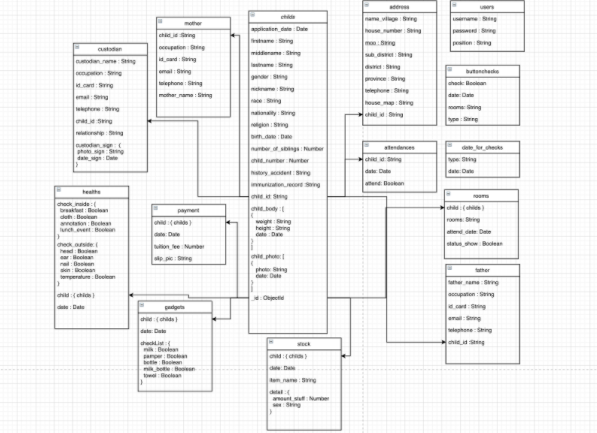
\includegraphics[width=140mm]{images/DiagramNursery2}
\end{center}
\caption[Poem]{Database Diagram}
\label{fig:walrus}
\end{figure}

\begin{figure}
  \begin{center}
  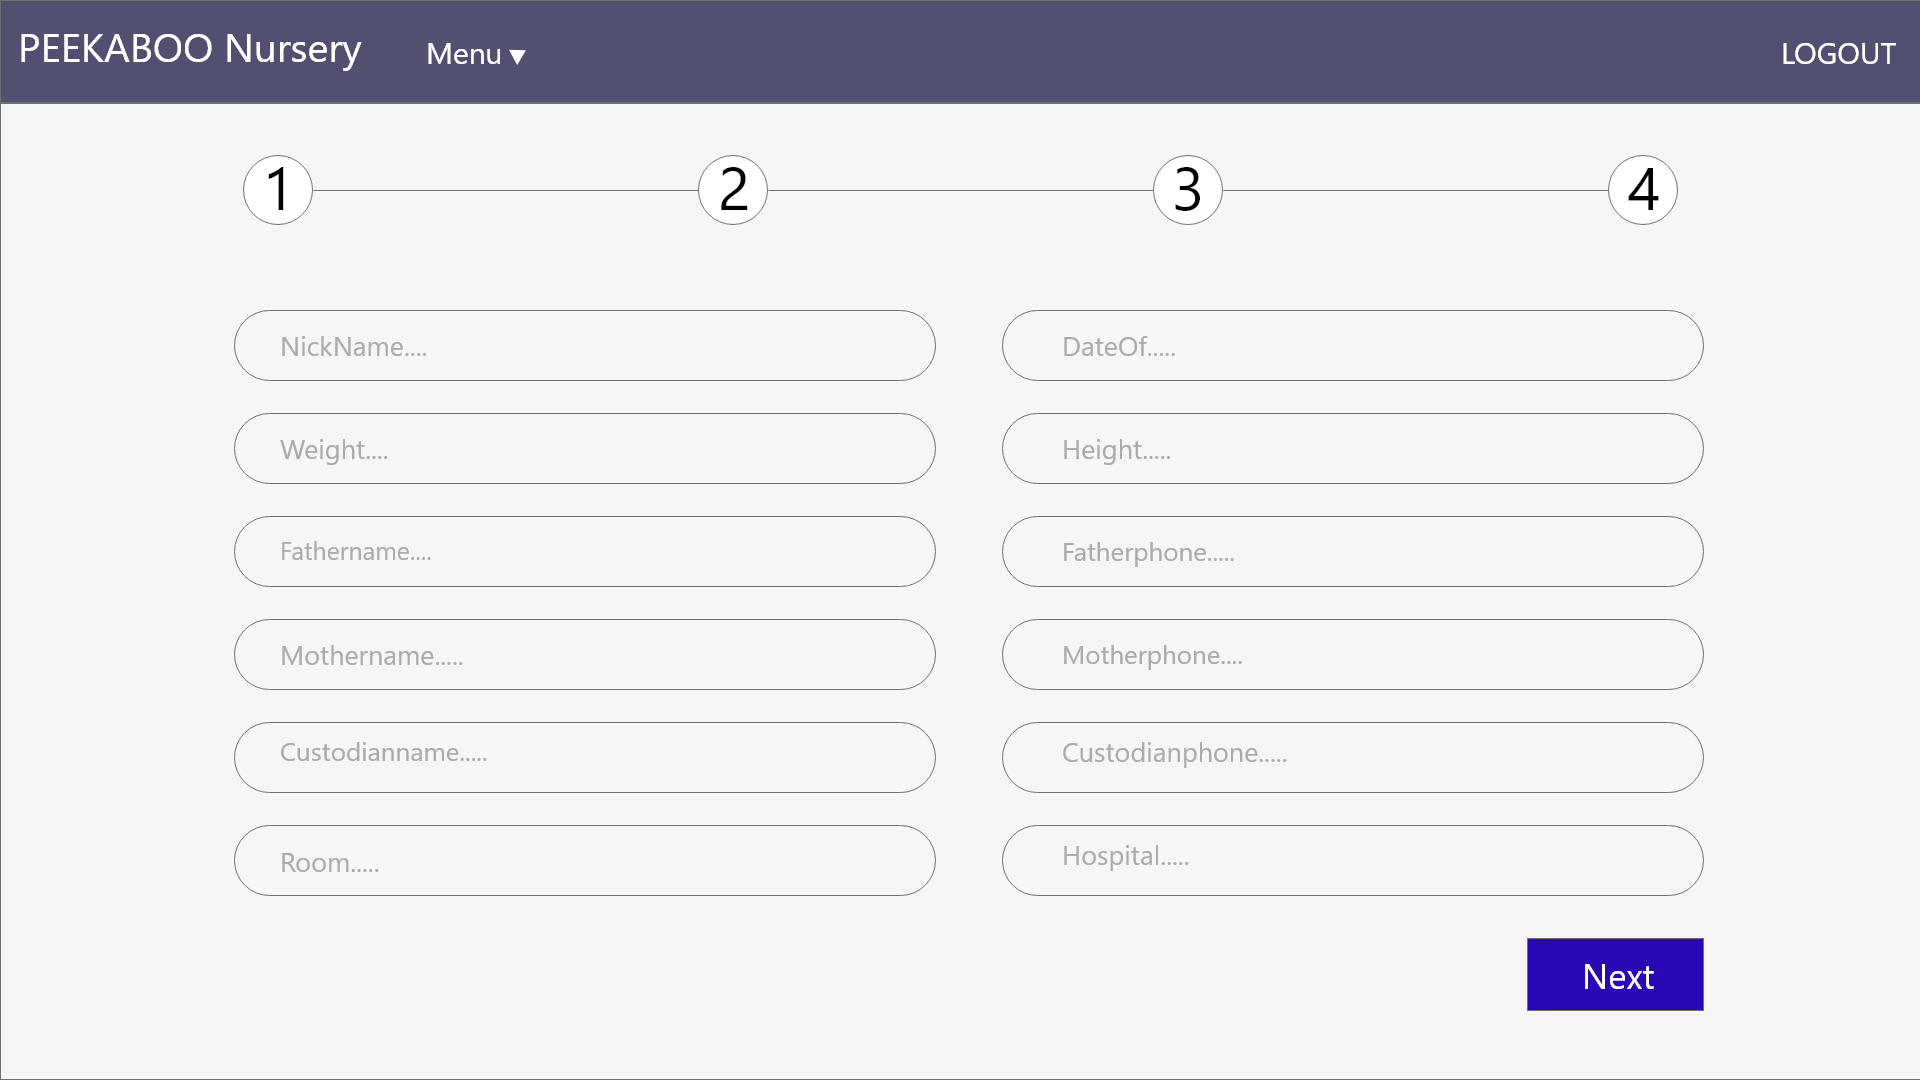
\includegraphics[width=140mm]{images/registerPage.png}
  \end{center}
  \caption[Poem]{Register Page}
  \label{fig:walrus}
  \end{figure}

\begin{figure}
  \begin{center}
  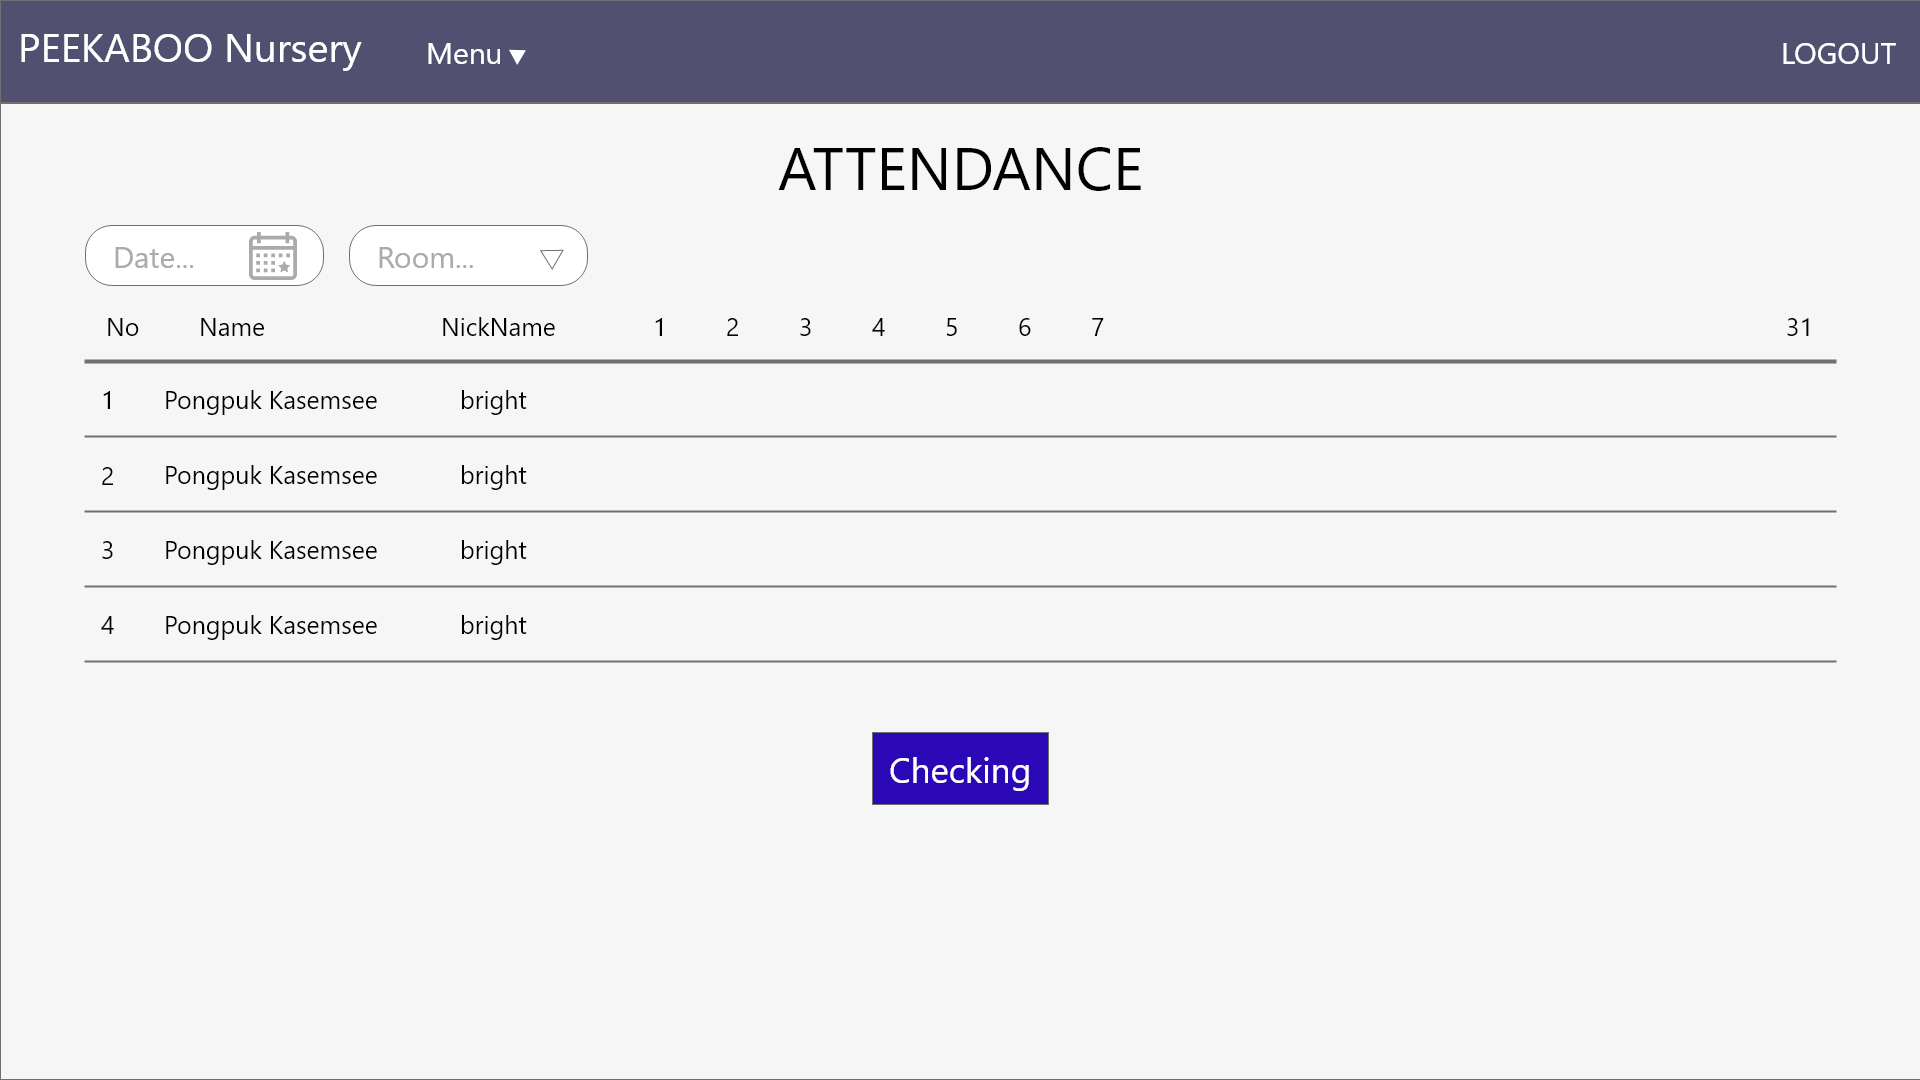
\includegraphics[width=140mm]{images/AttendancePage.png}
  \end{center}
  \caption[Poem]{Attendance Page}
  \label{fig:walrus}
  \end{figure}

\begin{figure}
  \begin{center}
  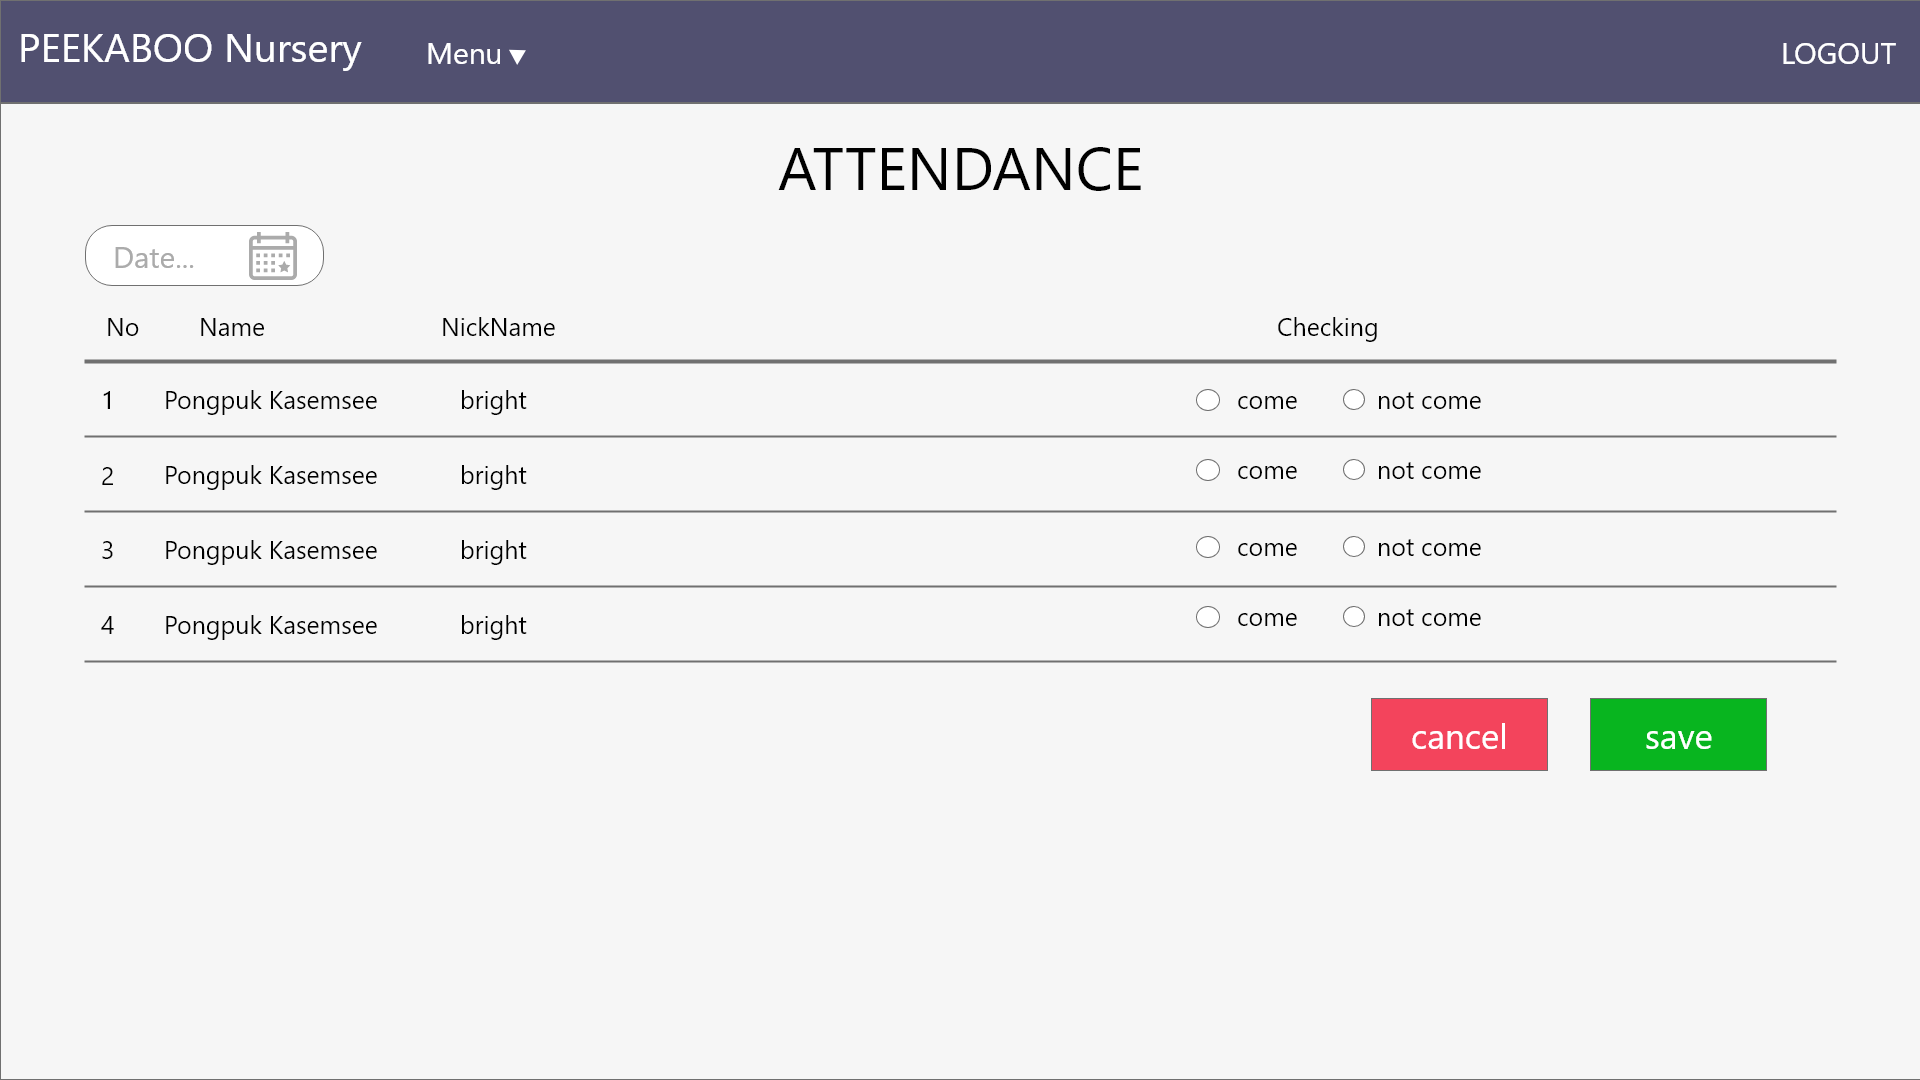
\includegraphics[width=140mm]{images/AttendancePageChecking.png}
  \end{center}
  \caption[Poem]{Check Attendance Page}
  \label{fig:walrus}
  \end{figure}

\begin{figure}
  \begin{center}
  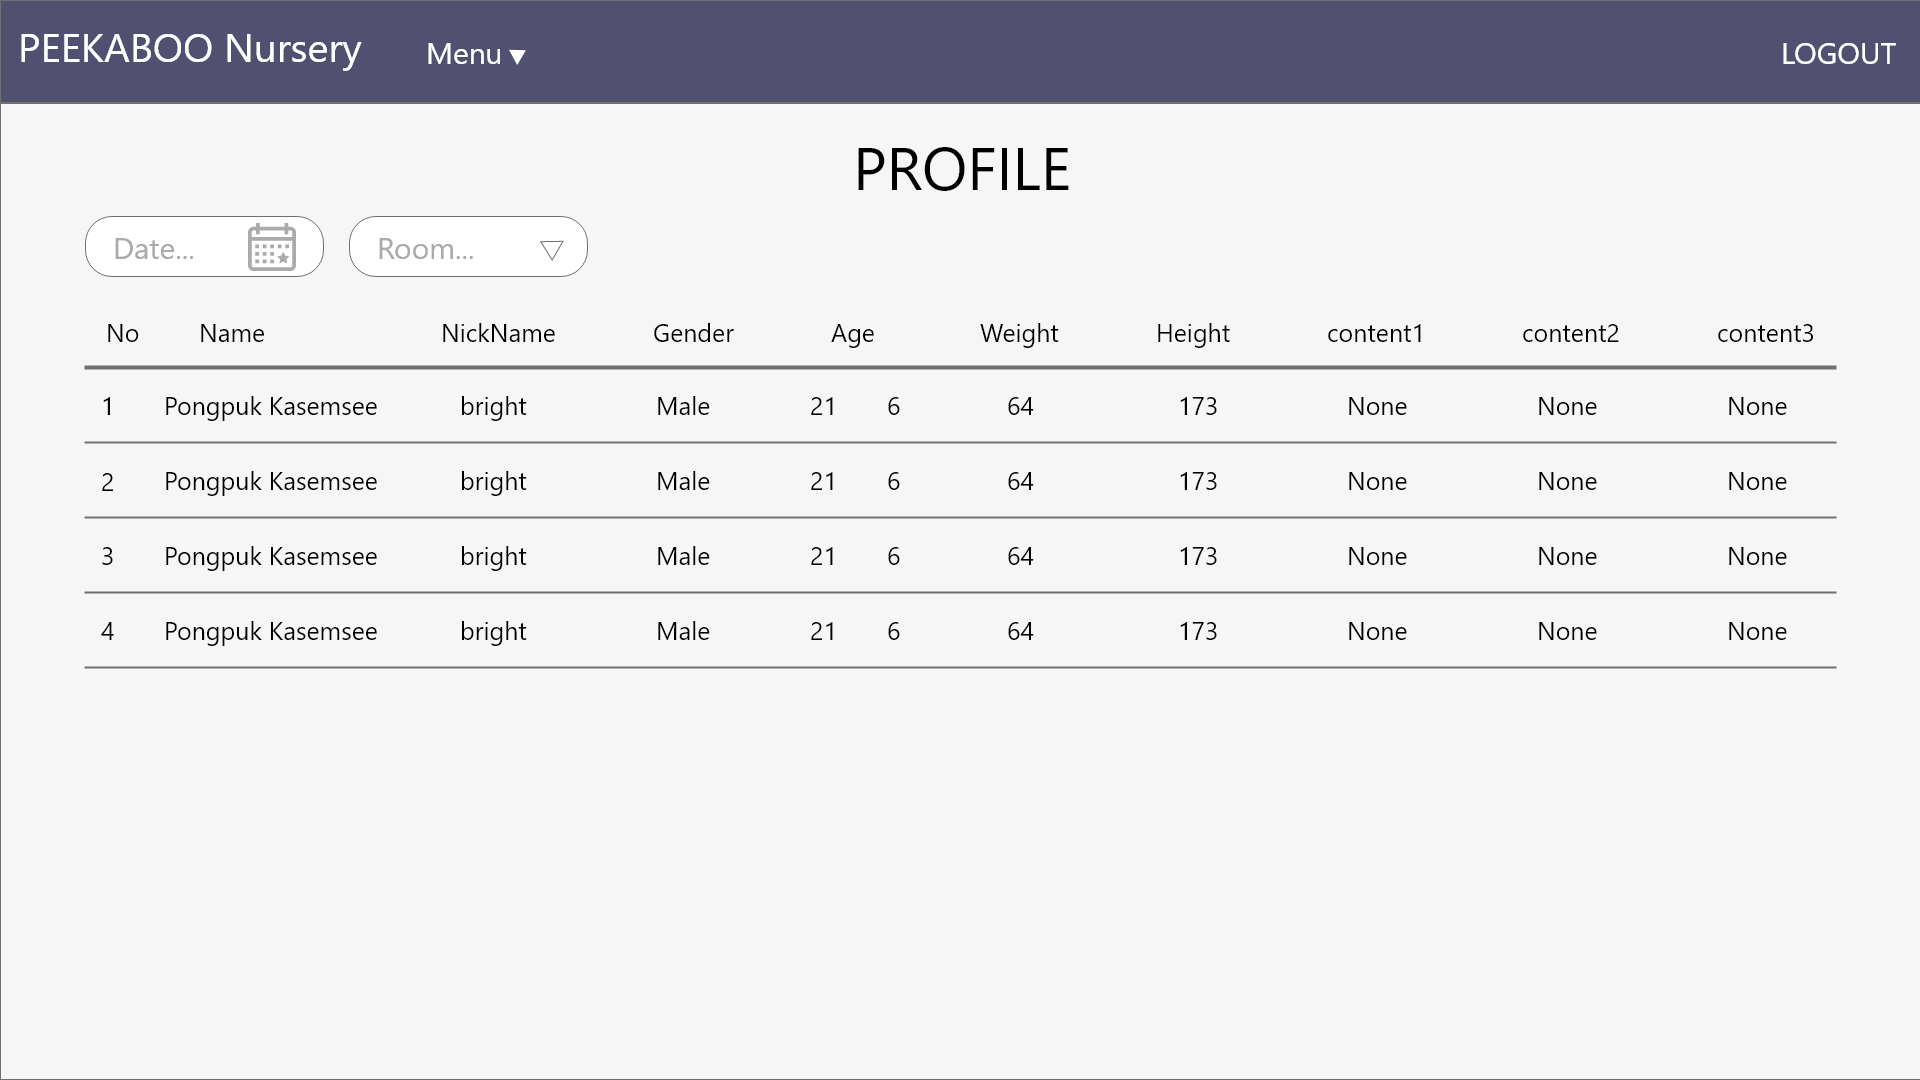
\includegraphics[width=140mm]{images/ProfileOnePage.png}
  \end{center}
  \caption[Poem]{Profile Page}
  \label{fig:walrus}
  \end{figure}

\begin{figure}
  \begin{center}
  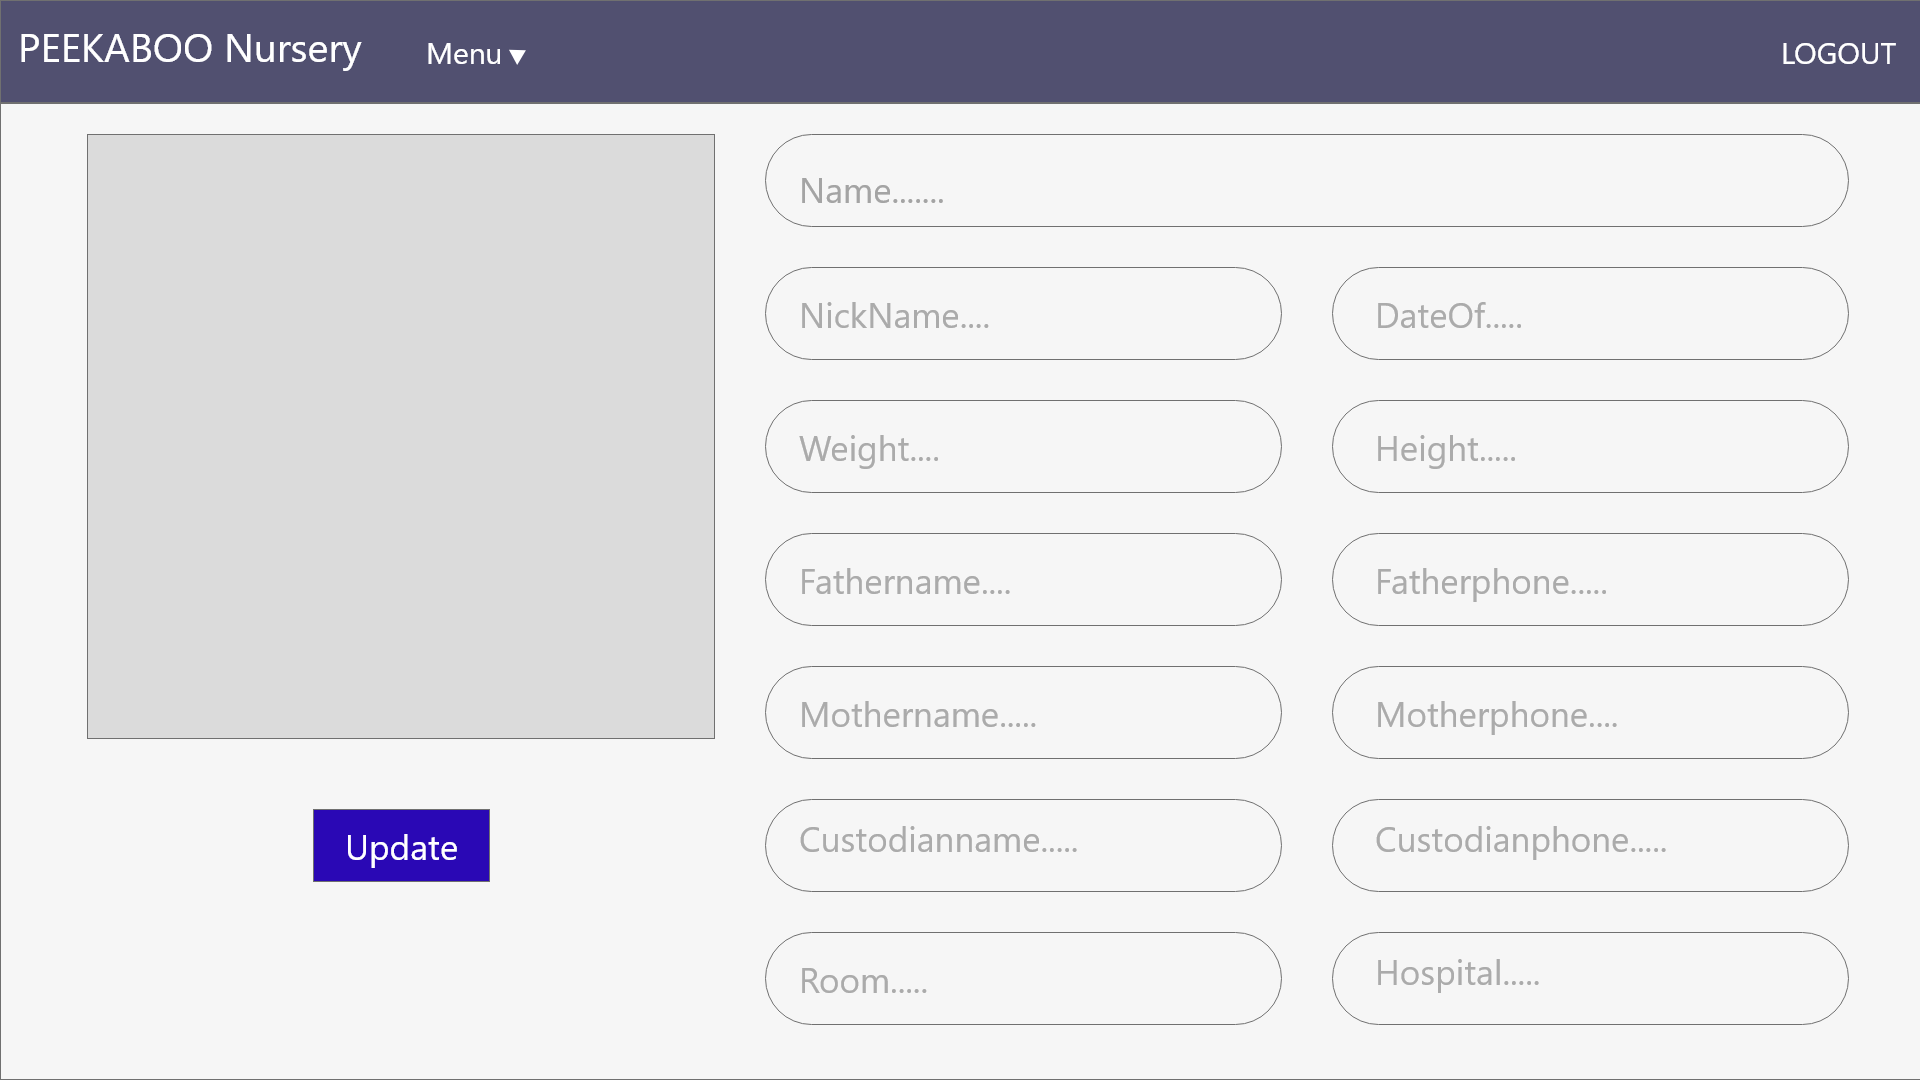
\includegraphics[width=140mm]{images/ProfileTwoPage.png}
  \end{center}
  \caption[Poem]{Profile Page}
  \label{fig:walrus}
  \end{figure}

\begin{figure}
  \begin{center}
  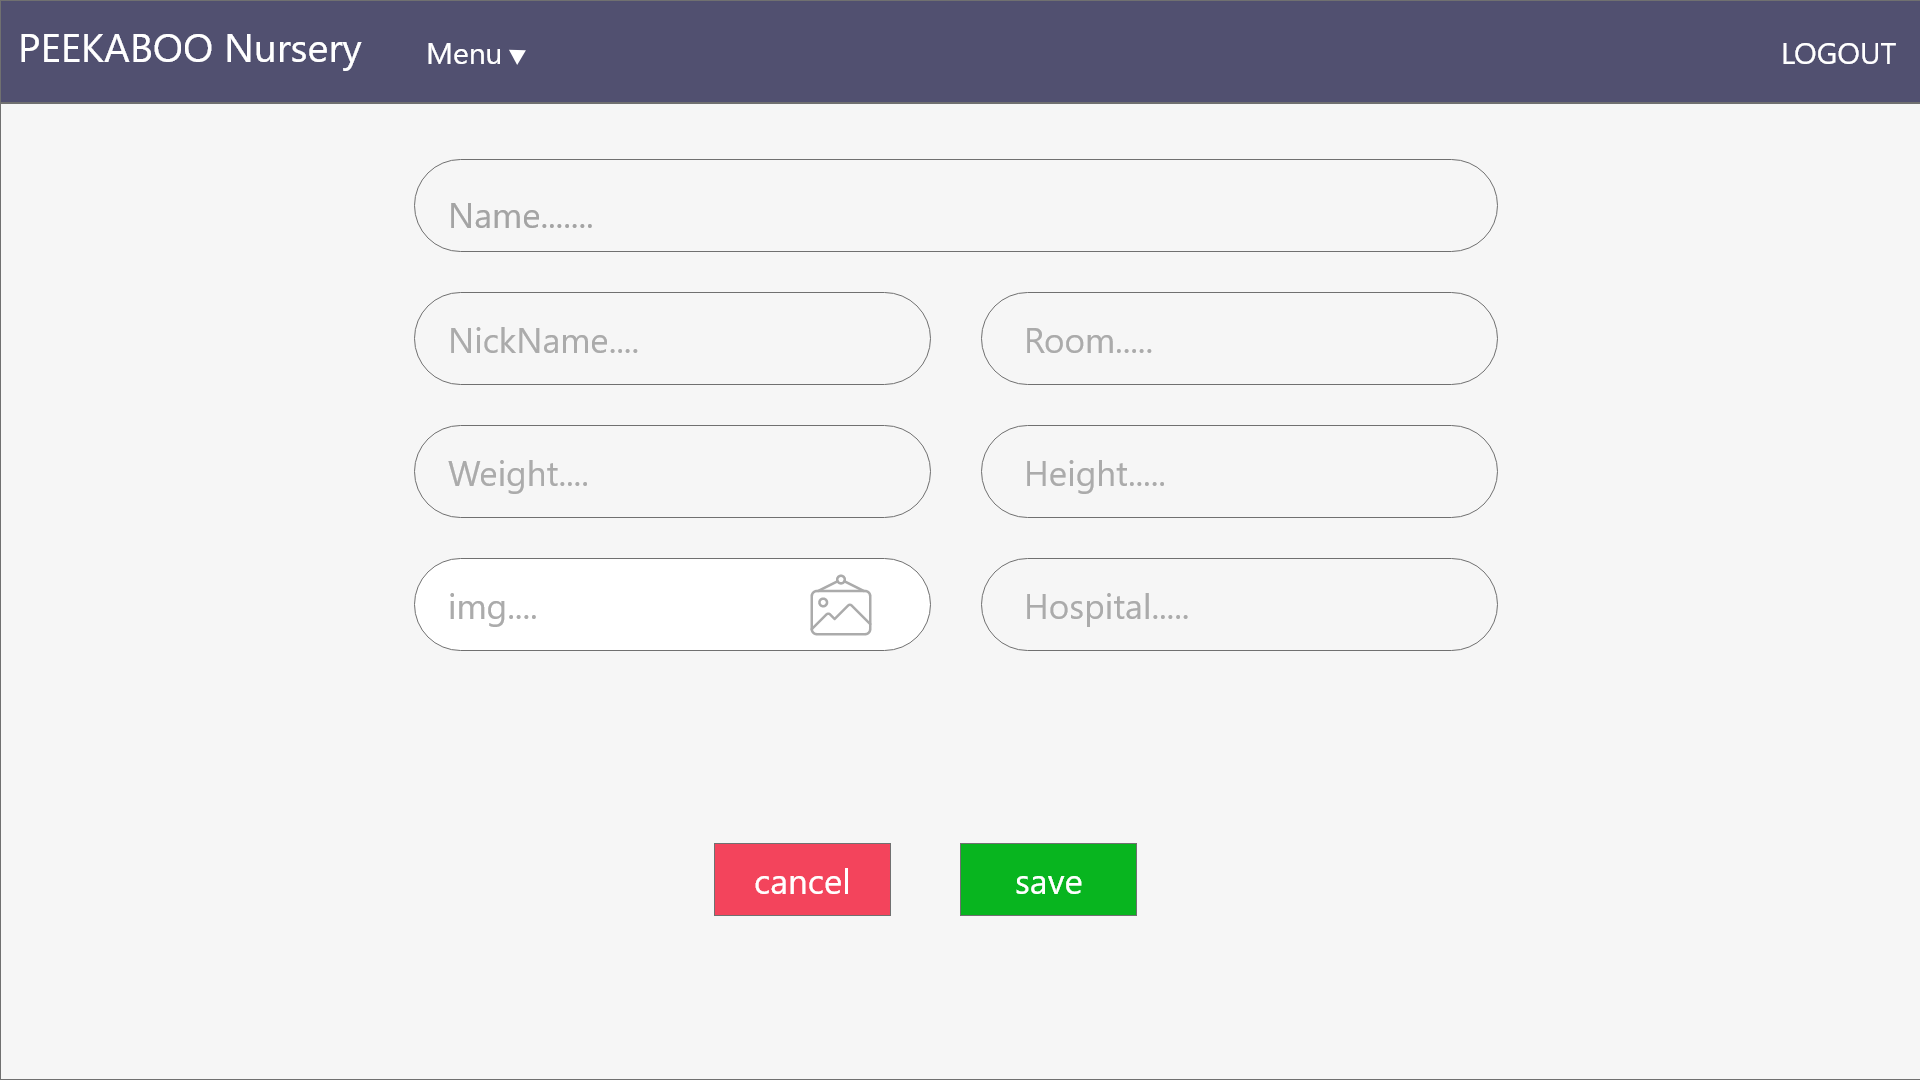
\includegraphics[width=140mm]{images/updateprofilePage.png}
  \end{center}
  \caption[Poem]{Update Profile Page}
  \label{fig:walrus}
  \end{figure}

\begin{figure}
  \begin{center}
  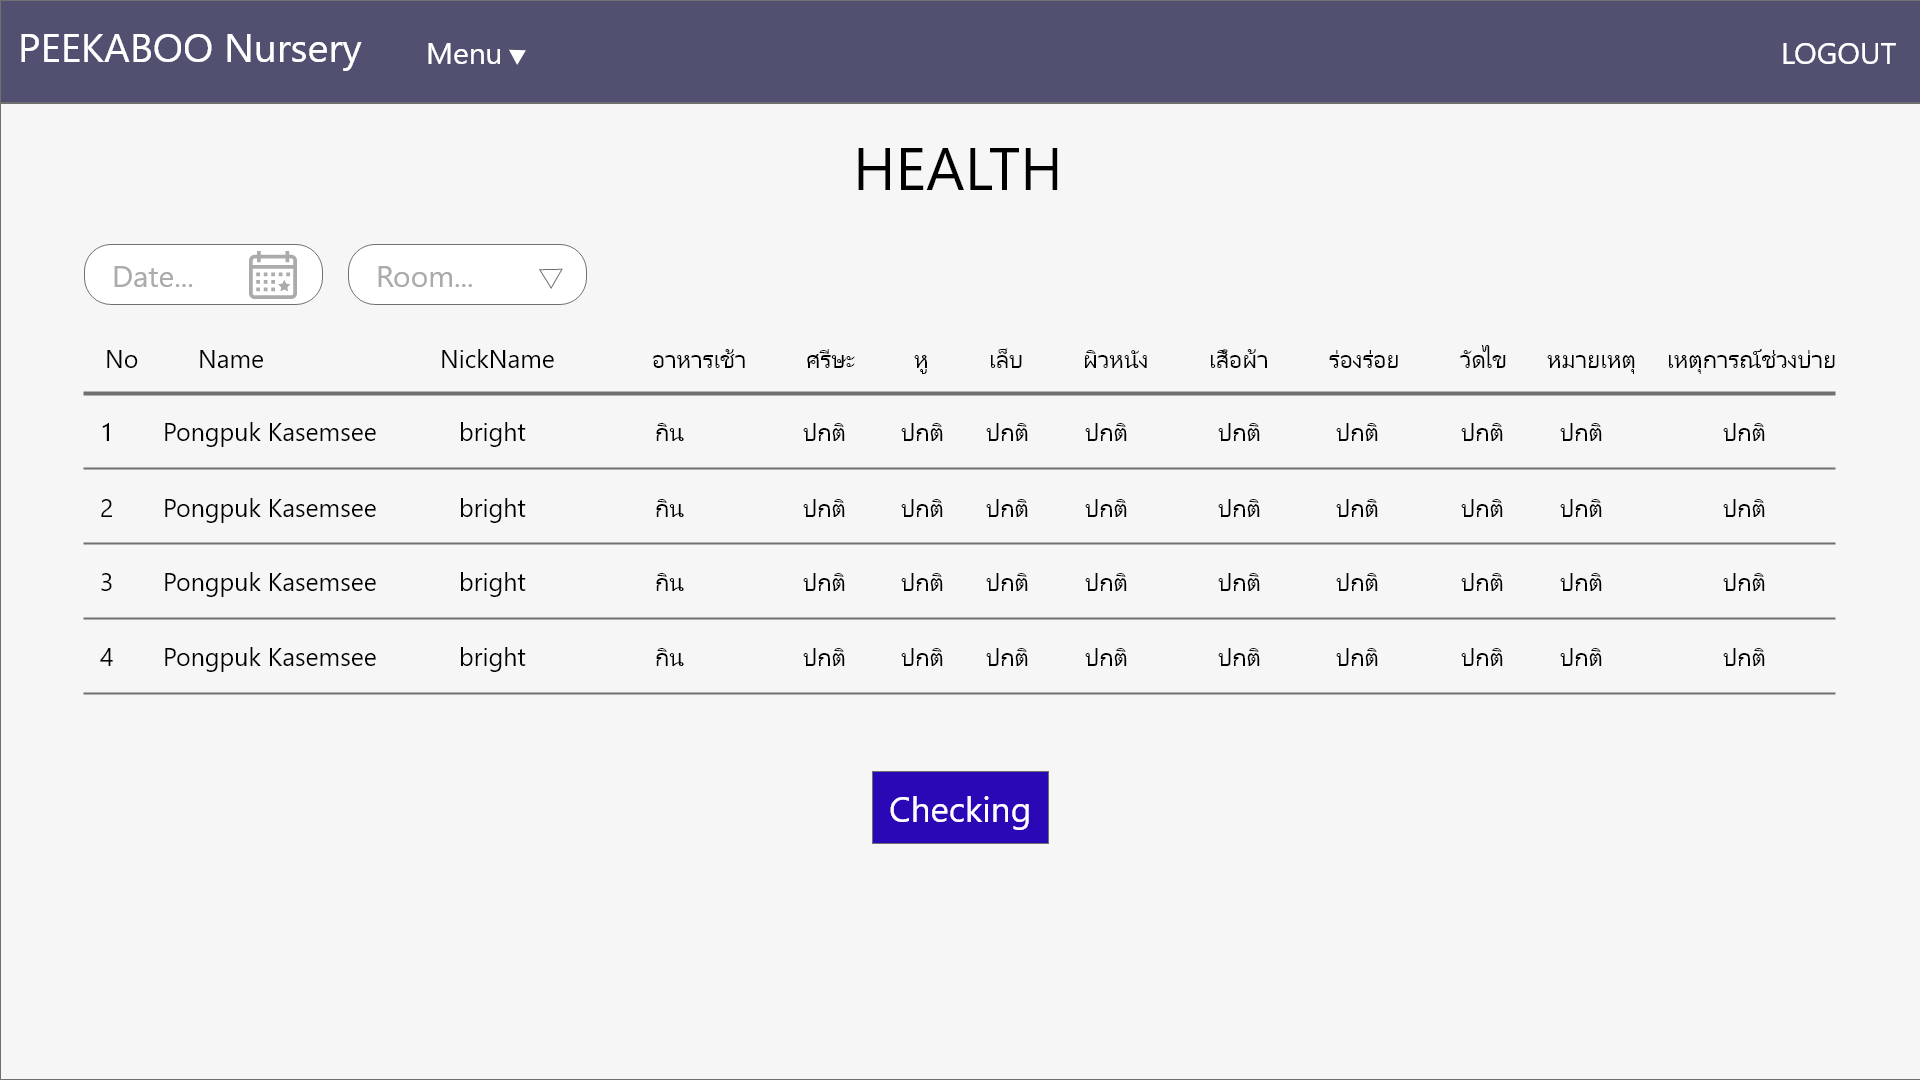
\includegraphics[width=140mm]{images/HealthPage.png}
  \end{center}
  \caption[Poem]{Health Page}
  \label{fig:walrus}
  \end{figure}

\begin{figure}
  \begin{center}
  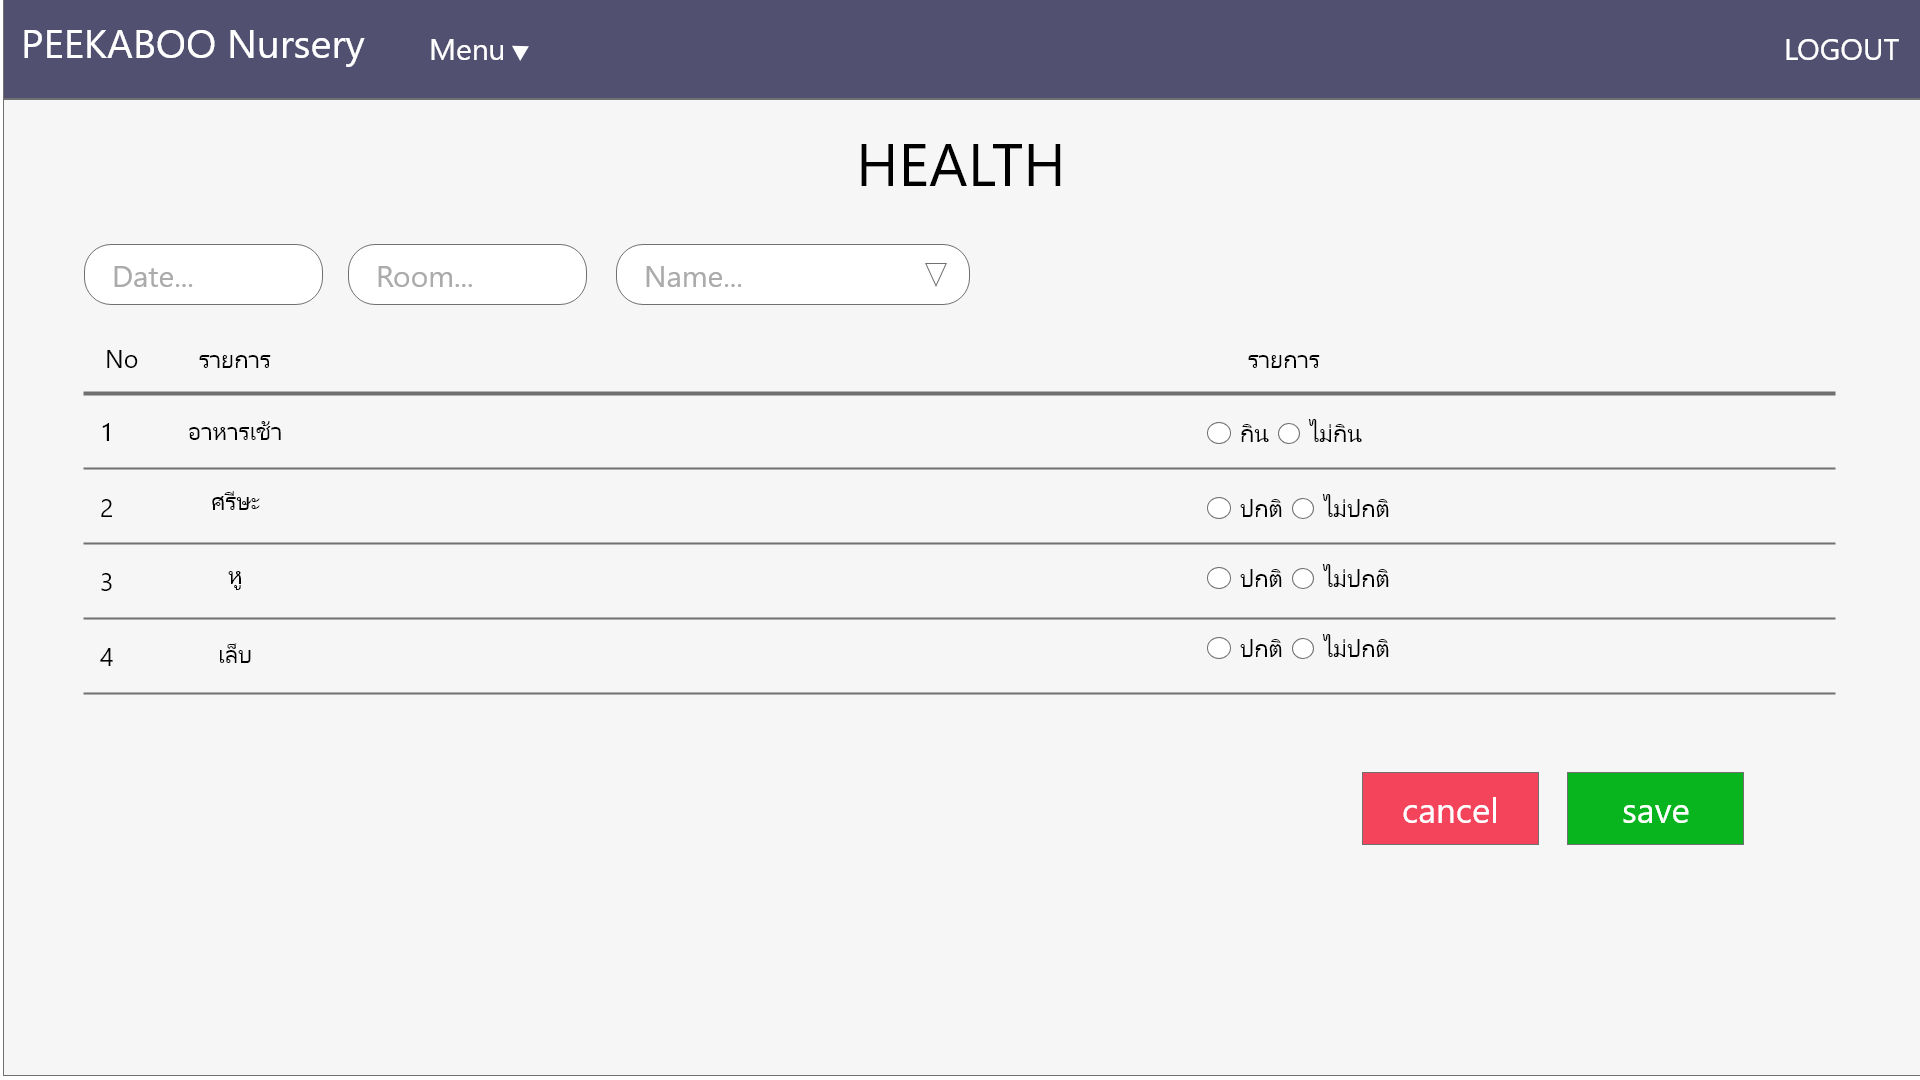
\includegraphics[width=140mm]{images/HealthPageChecking.png}
  \end{center}
  \caption[Poem]{Check Health Page}
  \label{fig:walrus}
  \end{figure}

\begin{figure}
  \begin{center}
  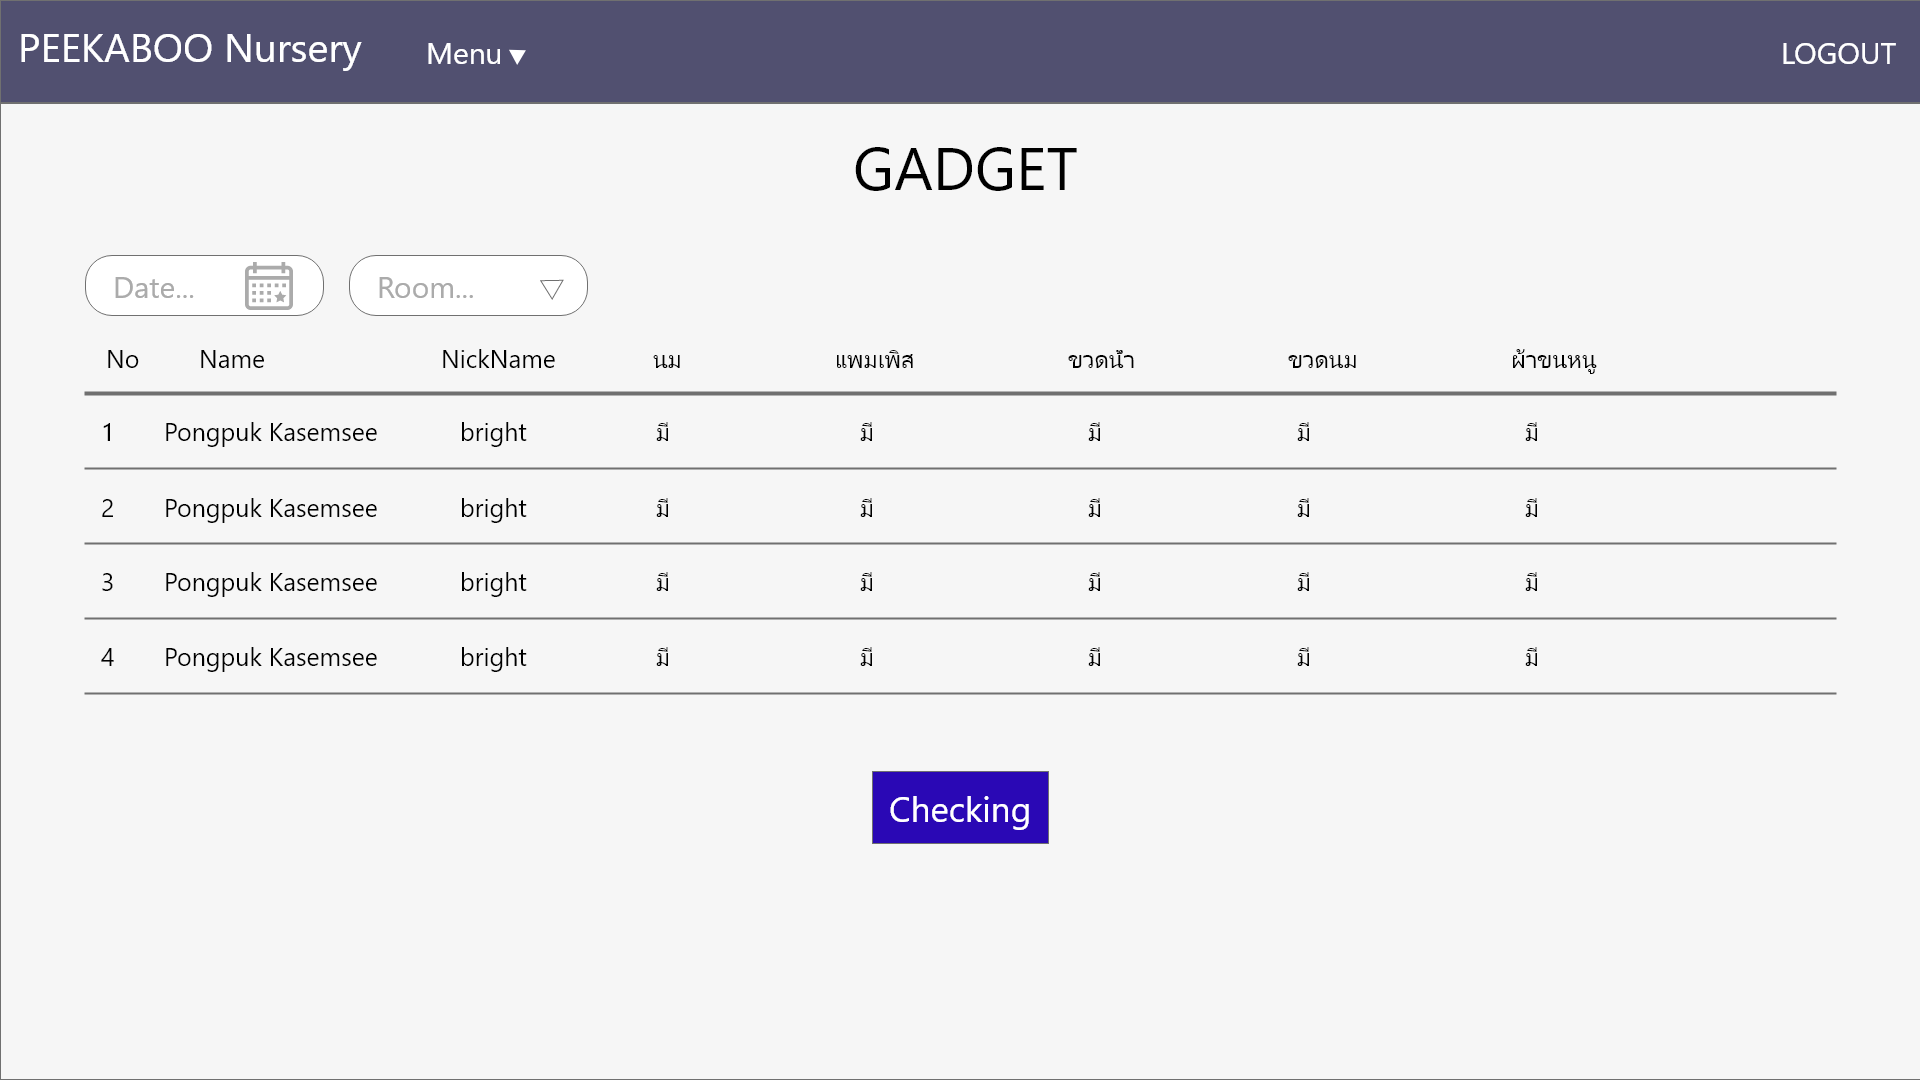
\includegraphics[width=140mm]{images/gadgetPage.png}
  \end{center}
  \caption[Poem]{gadget Page}
  \label{fig:walrus}
  \end{figure}

\begin{figure}
  \begin{center}
  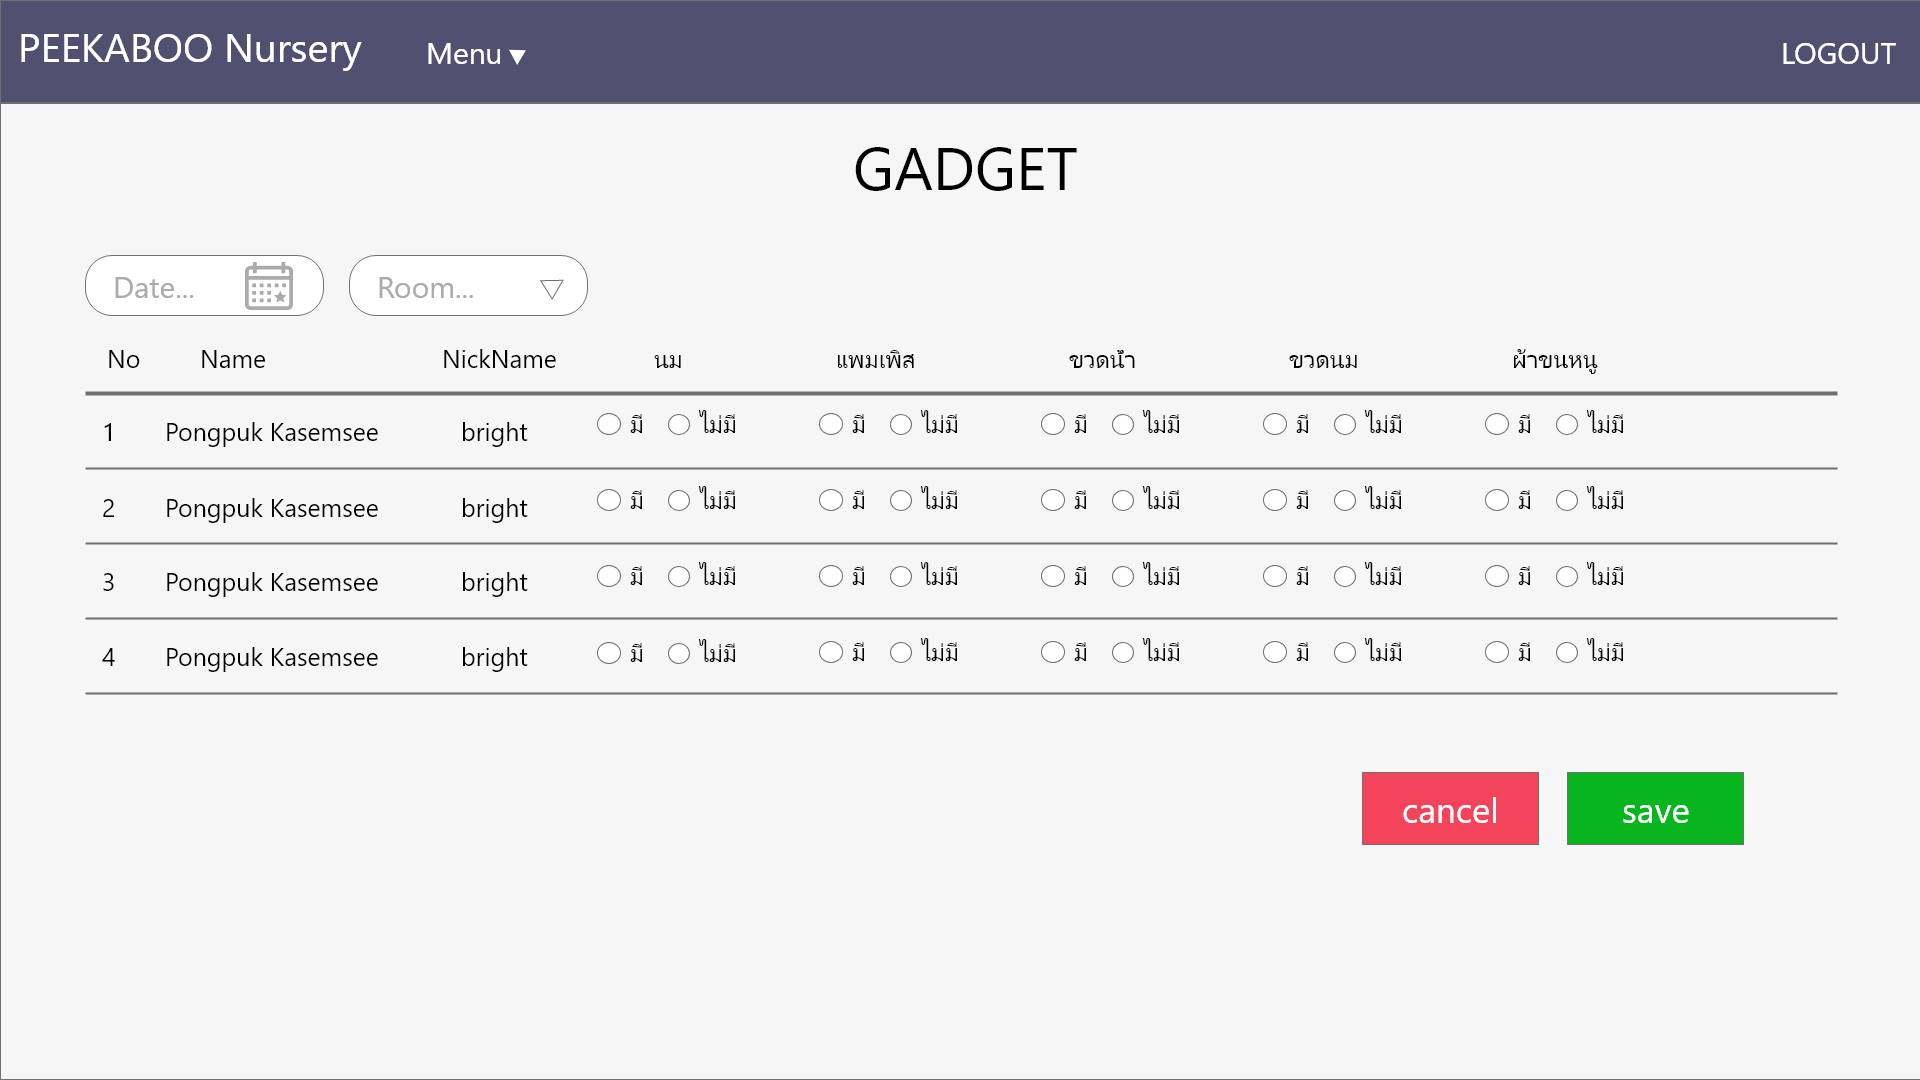
\includegraphics[width=140mm]{images/gadgetPageChecking.png}
  \end{center}
  \caption[Poem]{Check Gadget Page}
  \label{fig:walrus}
  \end{figure}

\begin{figure}
  \begin{center}
  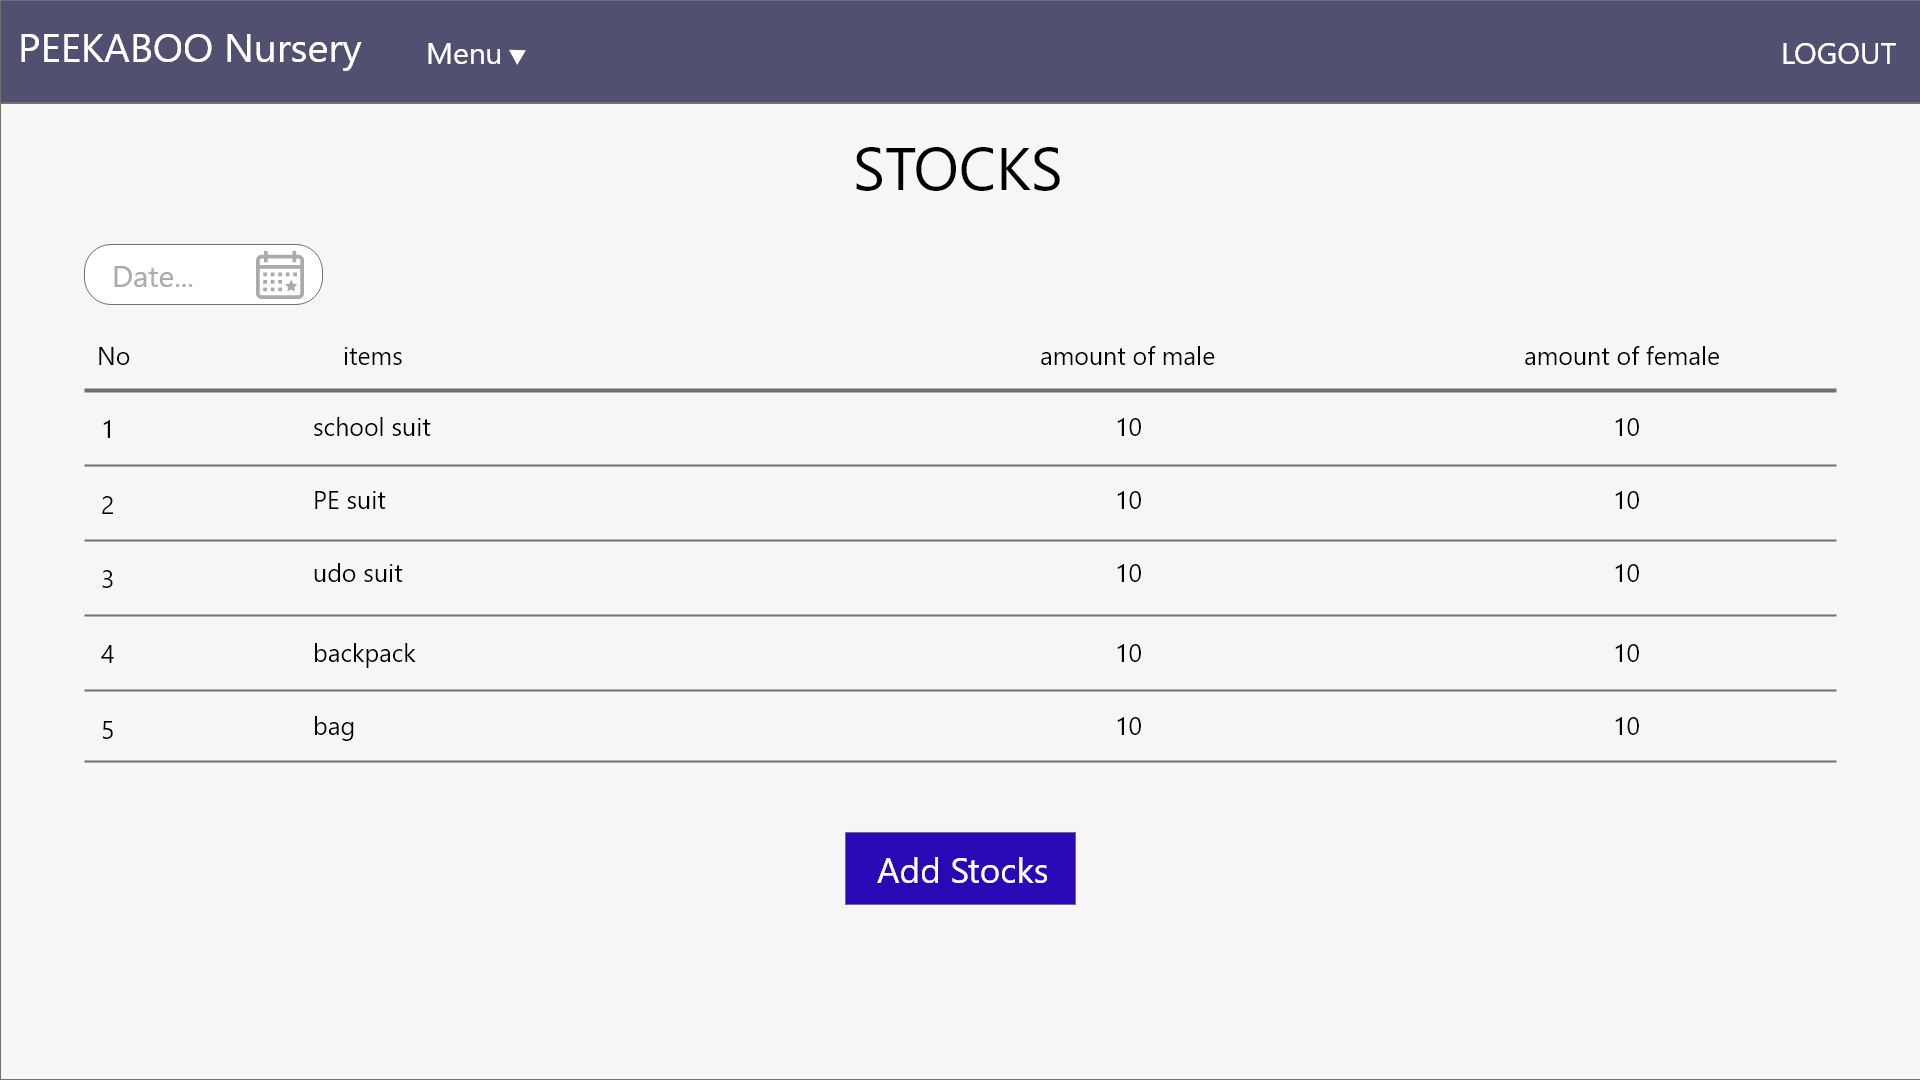
\includegraphics[width=140mm]{images/stockPage.png}
  \end{center}
  \caption[Poem]{Stock Page}
  \label{fig:walrus}
  \end{figure}

\begin{figure}
  \begin{center}
  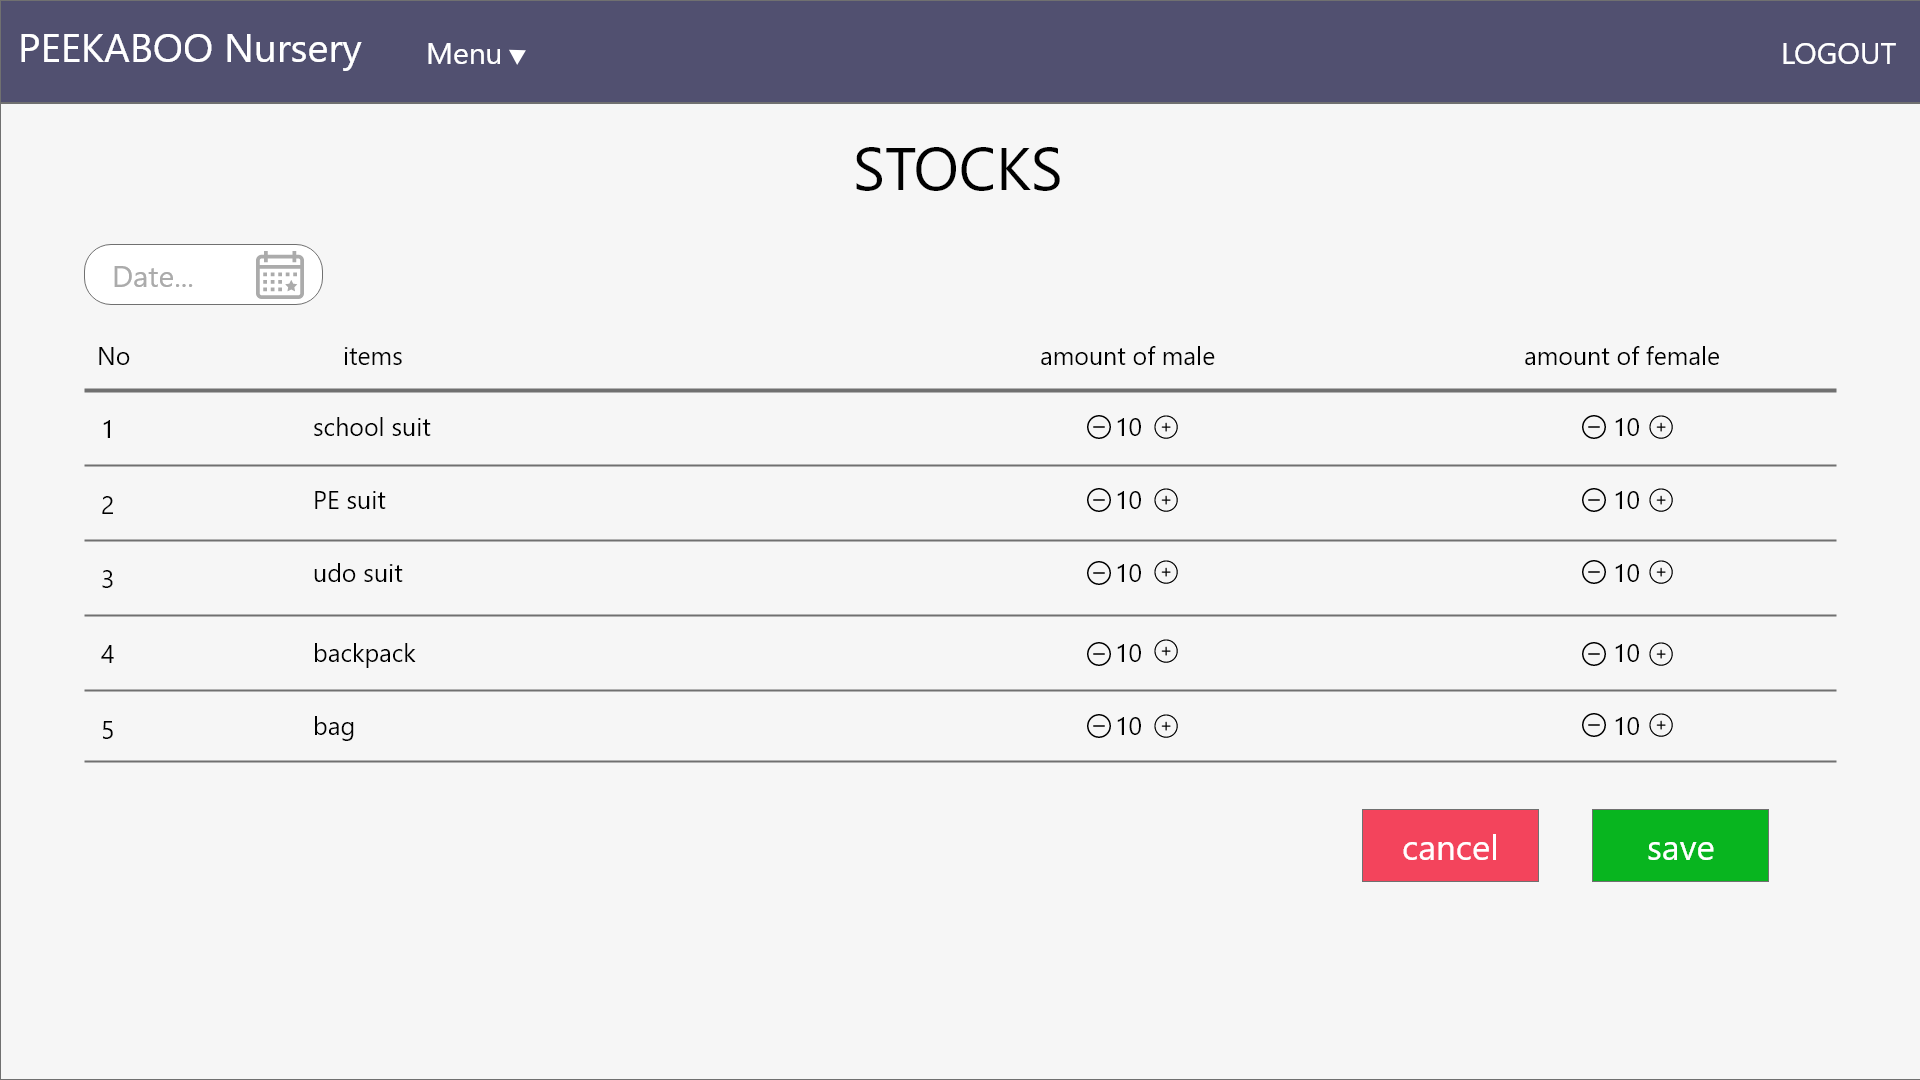
\includegraphics[width=140mm]{images/stockPageChecking.png}
  \end{center}
  \caption[Poem]{Check Stock Page}
  \label{fig:walrus}
  \end{figure}

\begin{figure}
  \begin{center}
  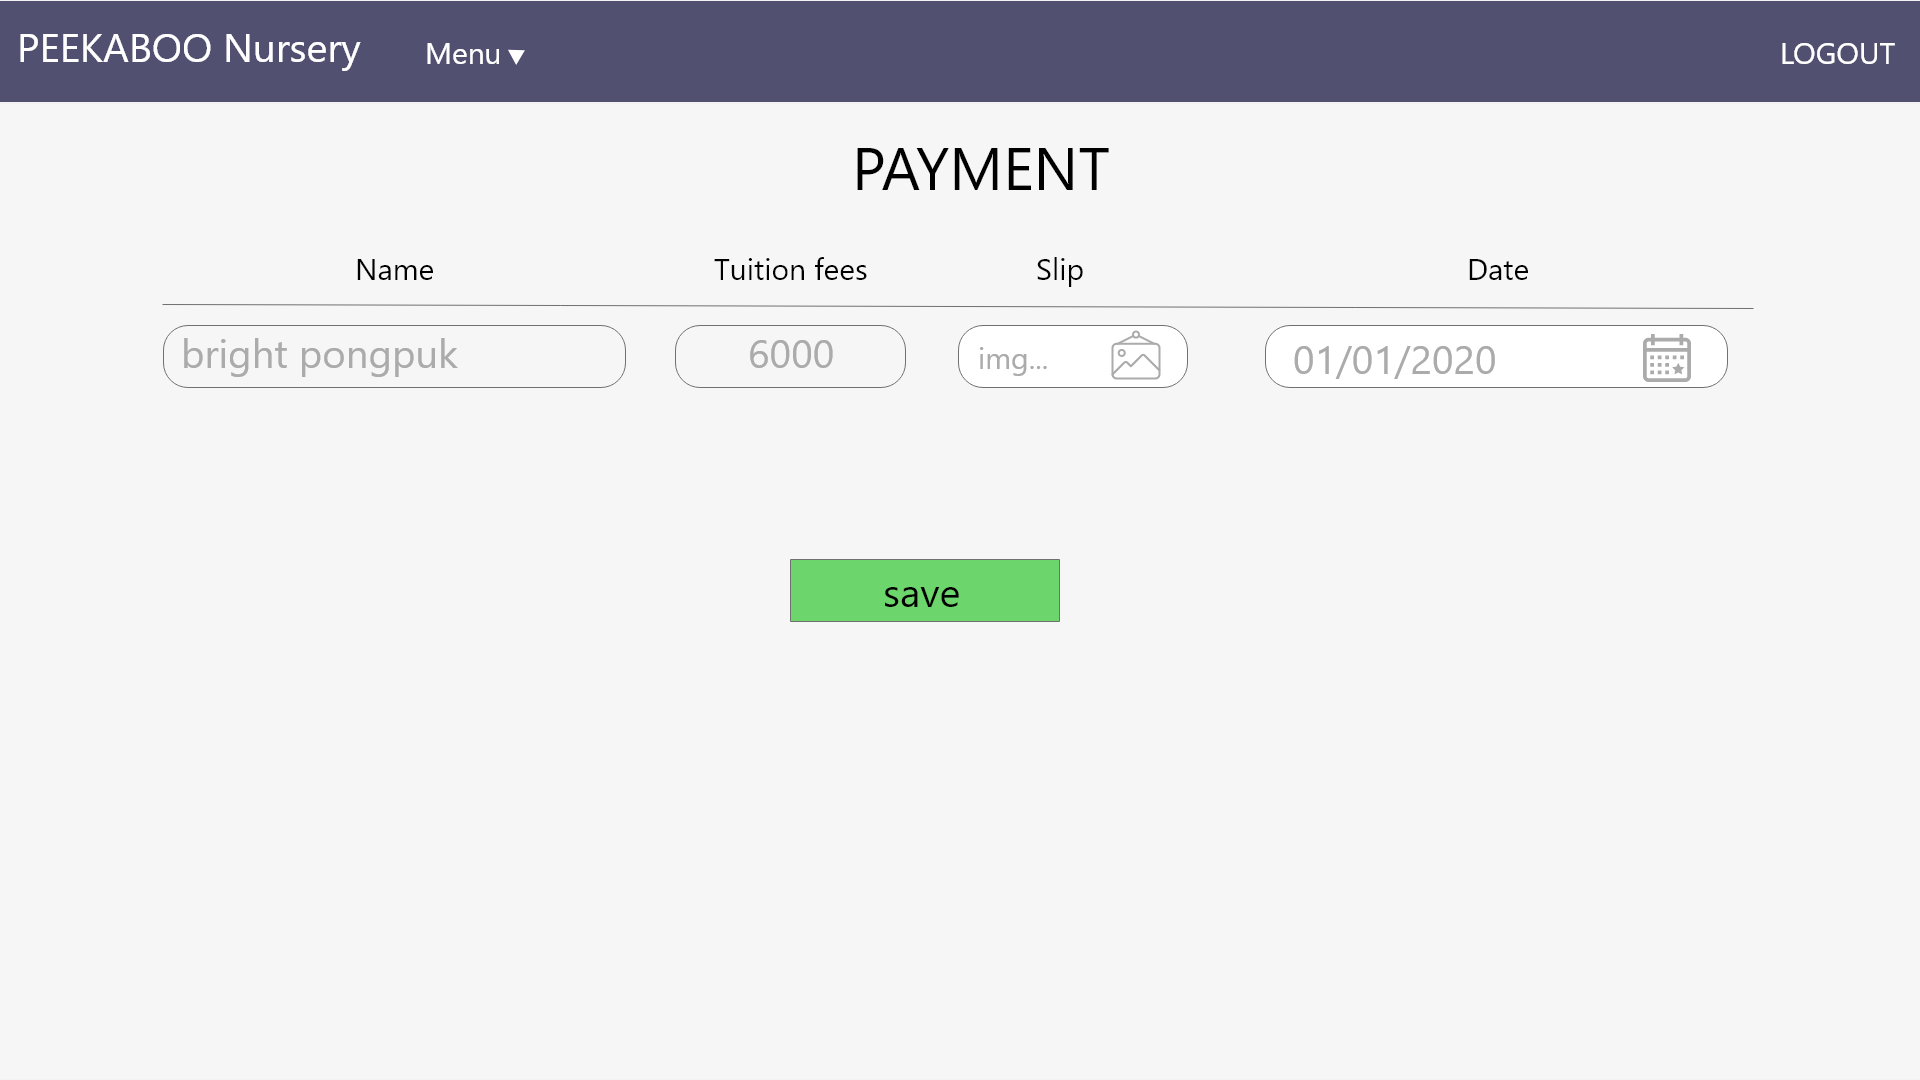
\includegraphics[width=140mm]{images/paymentPage.png}
  \end{center}
  \caption[Poem]{Payment Page}
  \label{fig:walrus}
  \end{figure}


\subsection{Database Diagram}
\begin{figure}
  \begin{center}
  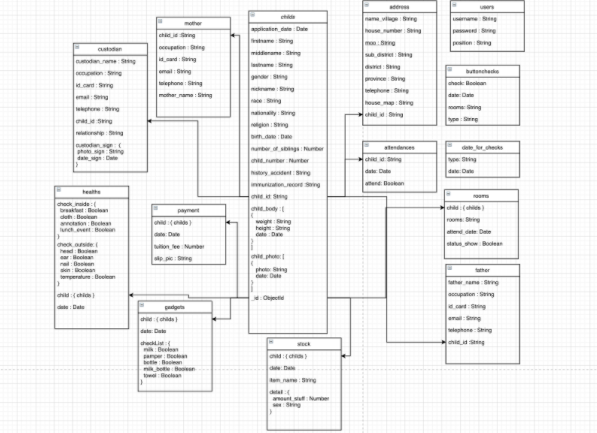
\includegraphics[width=140mm]{images/DiagramNursery2}
  \end{center}
  \caption[Poem]{Database Diagram}
  \label{fig:walrus}
  \end{figure}

\subsection{Architecture}
ระบบหลักๆที่ทางผู้พัฒนาใช้จะเป็นระบบแบบ Client-Server คือในทางฝั่ง Client จะใช้ React ในการพัฒนาแบบ Web-browser ให้ทางผู้ใช้ส่ง Requests มายังฝั่ง Server เพื่อที่จะทำงานต้องที่ผู้ใช้ต้องการ ซึ่งฝั่ง Server 
จะพัฒนาโดย Express.js ทางฝั่งนี้ก็จะ query ข้อมูลจากทางฐานข้อมูลที่เก็บไว้บน Mongodb Atlas เมื่อได้รับข้อมูลแล้วก็จะทำการส่ง Responses กลับไปยัง Client เพื่อให้ผู้ใช้สามารถทำงานในส่วนที่ต้องการได้ตามที่ต้องการ


\section{ขั้นตอนการดำเนินงาน}
\subsection{Discovery}
\begin{itemize}
  \item สำรวจและสอบถามปัญหาจากstakeholder
  \item นำปัญหาต่างหรือrequirementsมาวิเคราะห์
  \item สรุปผลแล้วนำrequirementsที่ได้จากการวิเคราะห์ไป  ทำต่อในขั้นตอนถัดไป
\end{itemize}
\subsection{Design}
\begin{itemize}
  \item ออกแบบหน้า UI/UX โดย Adobe XD
  \item ออกแบบฐานข้อมูลโดย Draw.io
  \item ออกแบบ
\end{itemize}
\subsection{Develop}
\begin{itemize}
  \item สร้าง Database
  \item เขียน Backend ตามที่ได้ Design มาในขั้นตอนก่อนหน้า
  \item เขียน Frontend แล้วทดสอบยิง Api ไปยังฝั่ง Backend
  \item เชื่อมโค้ด Frontend กับ Backend ผ่าน Api
\end{itemize}
\subsection{Testing}
